\section{Graph model and extraction}
\label{sec:graph_model}

Agentproof defines a framework-agnostic workflow representation,
\texttt{AgentGraph}, with typed nodes and edges. This abstraction is the common
surface for verification.

\subsection{Abstract model}
An \texttt{AgentGraph} consists of a set of nodes $V$, edges $E$, an entry node
identifier, and one or more exit identifiers. Each node has a \emph{kind}:
\texttt{ENTRY}, \texttt{EXIT}, \texttt{TOOL}, \texttt{LLM}, \texttt{ROUTER},
\texttt{HUMAN}, \texttt{SUBGRAPH}, or \texttt{PASSTHROUGH}. Each edge has a kind:
\texttt{DIRECT}, \texttt{CONDITIONAL}, \texttt{PARALLEL}, or \texttt{LOOP}.

Tool nodes may include a list of bound tool names (e.g., \texttt{("http\_get",
"s3\_download")}). Edges may include optional condition labels for conditional
branches.

\subsection{Framework extractors}
Agentproof includes extractors that map framework objects into this model:

\paragraph{LangGraph.}
LangGraph exposes a compiled state graph with sentinel start/end nodes. The
extractor identifies entry/exit sentinels, infers node kind from tool bindings
and naming heuristics (e.g., human review nodes), and encodes conditional edges
when the underlying framework marks an edge as conditional.

\paragraph{Google ADK.}
Google ADK composes agents as a tree of sequential, parallel, and loop agents.
The extractor performs a tree walk, emitting subgraph nodes for composite
agents and encoding sequential chains, parallel fan-outs, and loop back-edges.

\paragraph{AutoGen.}
AutoGen team topologies can be provided as a team object (e.g., round-robin) or
as an explicit list of agents plus a transition relation. The extractor
constructs a directed graph of speaker transitions, synthesizes entry/exit, and
connects leaf speakers to exit.

\paragraph{CrewAI.}
CrewAI describes task pipelines (sequential or hierarchical). The extractor
creates a node per task, uses process mode to add sequential edges or manager
routing edges, and incorporates context dependencies between tasks.

\subsection{Example workflow graph}
Figure~\ref{fig:example_graph} shows a small extracted workflow used throughout
the paper to illustrate typed nodes and conditional branches.

\begin{figure}[t]
  \centering
  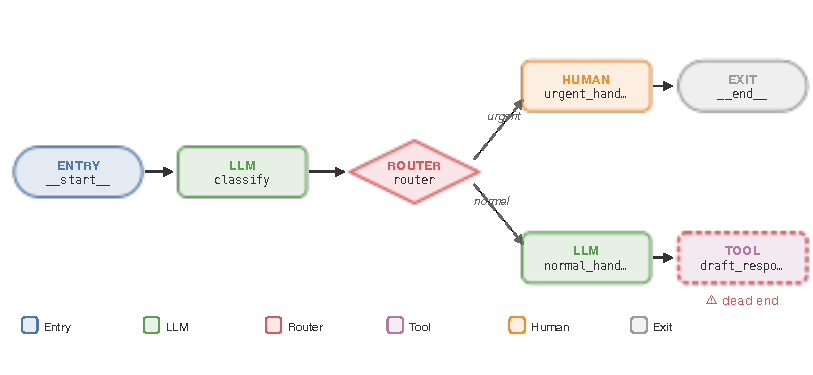
\includegraphics[width=\linewidth]{figures/example_graph.pdf}
  \caption{Example extracted workflow graph with typed nodes (ENTRY/ROUTER/LLM/TOOL/HUMAN/EXIT).}
  \label{fig:example_graph}
\end{figure}

